% Created 2023-11-23 Thu 01:06
% Intended LaTeX compiler: xelatex
\documentclass[11pt]{article}
\usepackage{graphicx}
\usepackage{longtable}
\usepackage{wrapfig}
\usepackage{rotating}
\usepackage[normalem]{ulem}
\usepackage{amsmath}
\usepackage{amssymb}
\usepackage{capt-of}
\usepackage{hyperref}
\usepackage{minted}
\usepackage[margin=2cm]{geometry}
\input{~/.doom.d/fancyLatexTemplate.tex}
\author{Spyridon Baltsas - AEM: 10443}
\date{}
\title{Parallel and Distributed Systems - Graph Minor Report}
\hypersetup{
 pdfauthor={Spyridon Baltsas - AEM: 10443},
 pdftitle={Parallel and Distributed Systems - Graph Minor Report},
 pdfkeywords={},
 pdfsubject={},
 pdfcreator={Emacs 28.2 (Org mode 9.6.1)}, 
 pdflang={English}}
\begin{document}

\maketitle

\section{Summary}
\label{sec:org953e5d6}
This report is about my proposed solution for the Graph Minor - Graph Grouping problem. More specifically, here will be briefly presented the algorithm that I have implemented for my approach, an estimate for its time complexity, its general efficiency in handling various datasets. In addition, we may see how it behaves when we use several Parallelization libraries and different number of threads each time. The source code and building instructions can be found (enter github link).
\section{The algorithm}
\label{sec:org5d84154}
The algorithm was designed with the following points in mind:
\begin{itemize}
\item Memory efficiency, since we may have to process very large datasets of sparse matrices with it
\item Time complexity, to make the most out the cycles of our CPU as possible
\item Parallelization. Split the data with the most efficient way possible, and keep the synchronization (mutexes/semaphores) at a minimum, without any data races of course
\end{itemize}
\subsection{Single Thread}
\label{sec:org8dd50ea}
The program takes as inputs 2 files, the first one contains the sparse matrix of the graph in matrix market (MM) format, and the second one is the vector c, which has information about which node belongs to which cluster, thus it has a length equal to the nodes of the graph. Equivalently, it has length equal to the amount of the non zero values in the adjacency matrix on the graph, in our case the sparse matrix in MM format. It stores the input matrix in COO format, but the Graph Minor's adjacency matrix in a format quite similar to CSC (in code this is an array of \texttt{struct row}), which contains the following data:
\begin{enumerate}
\item The non zero elements of the row (\texttt{int non\_zeros})
\item The columns which contain the non zero elements of the row as an array (\texttt{int *columns})
\item An array of the non zero values of the row (\texttt{int *values}).
\end{enumerate}
Let A the input sparse matrix of graph and M the sparse matrix of the desired graph minor. The program calculates the matrix minor without the need for matrix Ω of the specification, thanks to the following observation:
\begin{itemize}
\item The value of the i-th non zero element of A input matrix will be added up to the Graph Minor adjacency matrix element in row equal to c[rowsA[i]-1]-1 and in column c[colsA[i]-1]-1. Or, in other words:
\end{itemize}
\begin{equation}
\label{eq:1}
M[c[rowsA[i]-1]-1, c[colsA[i]-1]-1] += valuesA[i]
\end{equation}
The (-1)s are needed because we assume the matrix starts from 0 and not 1.
\subsection{Multi-threaded}
\label{sec:org419fb50}
The multi-threaded version of the algorithm use the same observation as above, but with some changes, in order to get parallelized effectively, without the need of synchronization using mutexes and signals. Therefore, we load each thread with a data structure (in code this is an array of \texttt{struct ThreadData}) containing the following information:
\begin{enumerate}
\item the ID of the thread (\texttt{int threadID})
\item The amount of matrix A's non zeros whose thread is responsible for (\texttt{int non\_zeros})
\item An array of indexes of the matrix A's non zeros (\texttt{int *non\_zeros\_indexes})
\end{enumerate}
We split the non zero elements of matrix A (COO format) to the responsible threads according to which row of the graph minor is element's destination. Each thread is responsible only for a distinct range of rows in the resulting graph minor matrix. Let N the number of available threads. Again, we assume that matrix starts from 0. Thus, for this job we use a modulo operation as seen in source code:
\begin{equation}
\label{eq:2}
c[rowsA[i] -1] -1 \mod{N}
\end{equation}
To be more clear, this is the part of the code which is responsible for this:
\begin{minted}[breaklines=true,breakanywhere=true,linenos=true,fontsize=\scriptsize]{c}
for(int i = 0; i < MAX_THREADS; ++i){
      threadData[i].threadID = i;
      threadData[i].non_zeros_indexes = malloc(NON_ZEROS_PER_THREAD[i]*sizeof(int));
      threadData[i].non_zeros = NON_ZEROS_PER_THREAD[i];
      counter = 0;
      for(int j = 0; j < NON_ZEROS; ++j){
          //split data among threads according to which row they belong in cluster adjacency matrix
          if((c[rowsA[j] -1 ] -1) % MAX_THREADS == i){
              threadData[i].non_zeros_indexes[counter] = j;
              counter++;
          }
      }
  }
\end{minted}
This way, each thread can process its data independently from each other, without any race conditions. This of course, adds a small overhead.
\subsection{Time complexity}
\label{sec:org4376f23}
Let n be the number of non zero elements of the input matrix, and m the number of non zero elements in the graph minor matrix. An approximation of the complexity of sequential algorithm would be \(\mathcal{O}(m\cdot n)\). In case of multi-threaded, would be \(\mathcal{O}{\left(\frac{m\cdot n}{N}\right)}\) where N is the number of available threads.
\section{Test Specifications}
\label{sec:org2eafd2a}
Please take note that on the following processing times the duration of the overhead was omitted. The following operations were considered as ``overhead'', as it may be seen from source code as well:
\begin{itemize}
\item I/O Operations. In our case, reading the data from the matrix market and vector files and printing to \texttt{stdout} the resulting sparse matrix.
\item Initialization of the required data structures before actually processing the input data.
\end{itemize}
\subsection{Technical Specifications}
\label{sec:org4ed4eb0}
The computer that was used to produce the following result times had the following specifications, processing power wise:
\begin{itemize}
\item Intel Core i5-8300H @ 2.30 GHz (4 cores, 8 threads)
\item 8GB DDR4 RAM @ 2667 MHz
\end{itemize}
Finally, the operating system was Debian Linux.
\subsection{Test Dataset Specifications}
\label{sec:org44f1675}
\begin{center}
\begin{tabular}{llll}
\hline
matrix name & rows & columns & non zero values\\[0pt]
\hline
ca2010.mtx & 710,145 & 710,145 & 3,489,366\\[0pt]
pa2010.mtx & 421,545 & 421,545 & 2,058,462\\[0pt]
ri2010.mtx & 25,181 & 25,181 & 125,750\\[0pt]
tx2010.mtx & 914,231 & 914,231 & 4,456,272\\[0pt]
nj2010.mtx & 169,588 & 169,588 & 829,912\\[0pt]
road usa.mtx & 23,947,347 & 23,947,347 & 57,708,624\\[0pt]
\hline
\end{tabular}
\end{center}
\section{Results}
\label{sec:org9ab3db7}
\subsection{Single Thread}
\label{sec:org755dadf}
\begin{center}
\begin{tabular}{|c|c|c|}
\hline
Datasets & Sequential time (seconds) & Matlab time (seconds)\\[0pt]
\hline
road usa.mtx & 2.429773 & 4.80690\\[0pt]
ca2010.mtx & 0.146844 & 0.12822\\[0pt]
pa2010.mtx & 0.081838 & 0.07003\\[0pt]
ri2010.mtx & 0.006248 & 0.00402\\[0pt]
tx2010.mtx & 0.181871 & 0.17025\\[0pt]
nj2010.mtx & 0.032843 & 0.02731\\[0pt]
\hline
\end{tabular}
\end{center}
\subsection{Multi-threaded}
\label{sec:org8b52f10}
The parallelization libraries that were used are according to the specification, P-threads, OpenMP and OpenCilk. The tests used 2,4,8,16,32,64 and 128 threads each time. It was noticed that above 128 there was no point of testing, because the result times were either similar to these ones of 128 threads or even worse, because the threads were too many for the processor to handle. In addition, a significant speedup is noticed when threads are between 4 and 8 , or even 4 and 16 in some cases, depending on the dataset. Last but not least it appears that OpenCilk is more efficient than the other two when we increase the number of threads and openMP tends to be a little more efficient than pthreads.
\pagebreak
\subsubsection{Charts}
\label{sec:org0c9582e}
Here are the result times of the parallel algorithm using the required libraries for various number of threads, summed up into charts.
\begin{center}
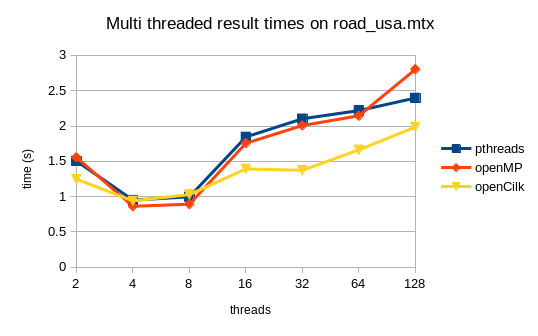
\includegraphics[height=180]{./charts/road_usa.png}
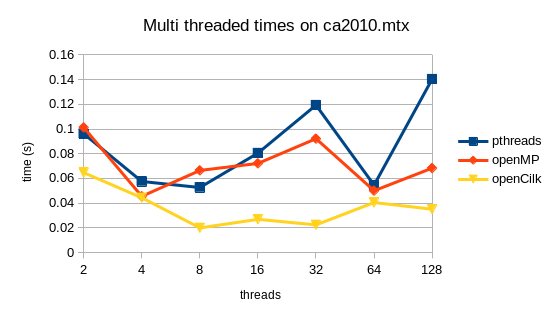
\includegraphics[height=180]{./charts/ca2010.png}
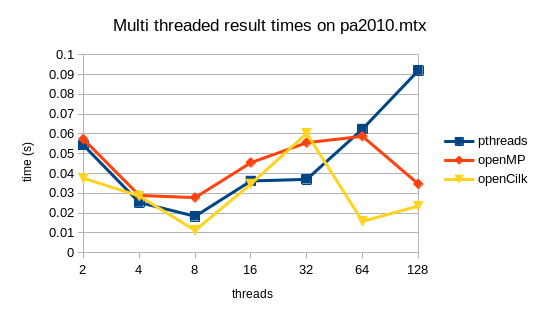
\includegraphics[height=180]{./charts/pa2010.png}
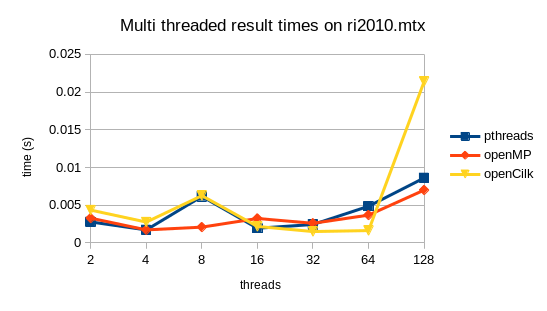
\includegraphics[height=180]{./charts/ri2010.png}
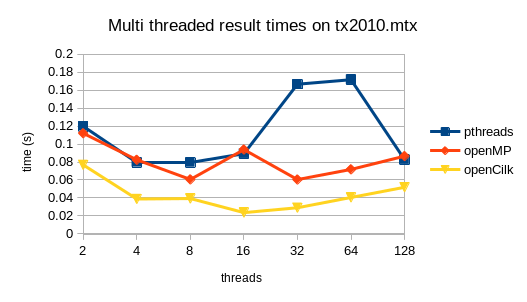
\includegraphics[height=180]{./charts/tx2010.png}
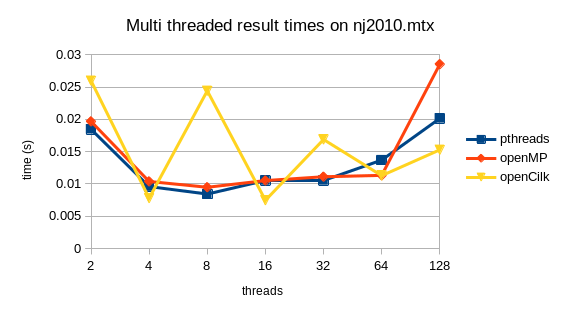
\includegraphics[height=180]{./charts/nj2010.png}
\end{center}
\end{document}